The developed tool provides a user interface for generating networks to simulate epidemics. To create these networks, different groups of people can be defined. Each group consists of $n$ nodes, the members, each of which has a certain number of edges to other nodes of the same group. The number of edges per node is determined by a mean $\mu$ and a delta $\delta$. Each node will then have an edge count between $\mu - \delta$ and $\mu + \delta$.

Let $g1$ and $g2$ be two different groups. Then in addition to the above mentioned edges within a group, it is also possible to specify the number of edges between the nodes of the two groups with an average and delta value, in the same way as described above.

To create a network graph that meets all of these requirements multiple algorithms are needed.

\section{Creating edges within a group}
\label{sec:creating_edges_in_group}
Let $g$ be a group of $n$ nodes, each of which needs between $\mu - \delta$ and $\mu + \delta$ edges. Then the first step is to generate a sequence of $n$ integer numbers within this range. This sequence represents the degree each node should have at the end.

\subsection{Randomly adding new edges}
\begin{algorithm}
\caption{Adding random edges}
\label{alg:random_edges}
\begin{algorithmic}
\State $nodes \gets $nodes with less than required degree
\While{$nodes$ is not empty}
    \State $n1, n2 \gets$ two unconnected nodes
    \State connect $n1$ and $n2$
    \If {$n1$ has required degree}
        \State remove $n1$ from $nodes$
    \EndIf
    \If {$n2$ has required degree}
        \State remove $n2$ from $nodes$
    \EndIf
\EndWhile
\end{algorithmic}
\end{algorithm}

This algorithm was the first iteration for creating the networks, it has two issues. 
\newline

First, not every sequence of degrees is graphic, e.g. not every sequence of degrees has a corresponding simple graph. A simple graph is a graph consisting only of undirected edges and no loops.

For example, let $s$ be a sequence of random integers with sum $m$. If $m$ is not even, $s$ is definitely not graphic, because in a simple graph without loops, every edge increases the total degree of all nodes by two. Thus it is impossible to have a total degree of all nodes that is not even. This is not checked in the above algorithm \ref{alg:random_edges}, which would cause the $nodes$ list to contain only one node at the end, making it impossible to select two unconnected nodes from it.
\newline

The second issue is that by adding edges randomly it is possible to end up in a situation, where all remaining edges are already connected but have still not reached the required degree.

\begin{figure}
    \centering
    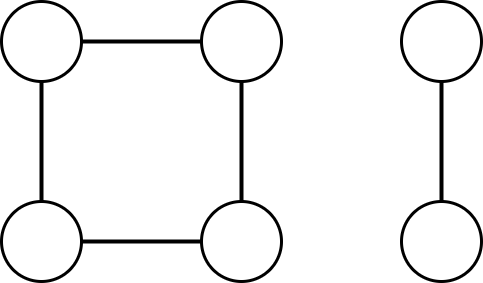
\includegraphics[width=0.5\linewidth]{images/impossible_graph.png}
    \caption{Graph created by random algorithm \ref{alg:random_edges} with $\mu=2$ and $\delta=0$}
    \label{fig:impossible_graph}
\end{figure}

Figure \ref{fig:impossible_graph} shows one such situation. In this graph each node needs to have a degree of exactly two. In theory it is possible to create such a graph, but the random algorithm \ref{alg:random_edges} may end up in the situation shown in the figure. Here the only two nodes remaining in the $nodes$ list are the two on the right which are already connected. From this state it is impossible to create a graph that satisfies the degree requirements.
\newline

The second iteration of the algorithm uses a more methodical approach to adding the edges to solve the above issues.

\subsection{Erdos-Gallai Theorem}
To solve the first problem of degree sequences that are not graphic, the Erdos-Gallai Theorem is used. It provides one of the two known approaches to solving the graph realization problem, i.e. it gives a necessary and sufficient condition for a finite sequence of natural numbers to be the degree sequence of a simple graph.

\begin{equation}
\sum_{i=1}^{k} d_i \leq k(k-1) + \sum_{i=k+1}^{n} \min(k, d_i)
\end{equation}
for all integers \(k\) with \(1 \leq k \leq n\), where \(d_1 \geq d_2 \geq \ldots \geq d_n\) are non-negative integers.

A sequence of degrees is graphic if and only if \(d_1 + d_2 + \ldots + d_n\) is even and the above equation holds for every $k$. The inequality ensures that the sum of the first $k$ terms of the degree sequence does not exceed the theoretical maximum number of edges $(k(k-1))$ plus the sum of the remaining edges $\sum_{i=k+1}^{n} \min(k, d_i)$ for the remaining vertices.

For this tool, every degree sequence needs to be graphic, because it should always be possible to generate a graph for the user's input. This means that if the Erdos-Gallai Theorem shows that a sequence is not graphic, it must be changed until it is. This is done by simply decrementing a random number of the degree sequence by one.

If the Erdos-Gallai Theorem failed because the sum was not even, the sum will be even after decrementing once. By decrementing random numbers of the sequence, only the left side of the inequality gets smaller, because $k$ never changes. This means after decrementing enough times, the theorem will always be fulfilled. Thus, any sequence of degrees can be changed to be graphic.

The python implementation of this algorithm can be seen in \ref{lst:erdos_gallai}.

\begin{lstlisting}[language=python, caption={Erdos-Gallai Theorem in Python}, label={lst:erdos_gallai}]
def _erdos_gallai(self) -> bool:
    if sum(self.deg_seq) % 2 != 0:
        return False
    n = self.size
    for k in range(1, n + 1):
        if sum(self.deg_seq[:k]) > k * (k - 1) + sum(min(k, d) for d in self.deg_seq[k + 1 :]):
            return False
    return True
\end{lstlisting}

\subsection{Havel-Hakimi algorithm}
\label{sub:havel_hakimi}
After creating a graphic degree sequence using the Erdos-Gallai Theorem, with all degrees within the $\mu - \delta$ and $\mu + \delta$ range, this degree sequence needs to be converted to a network graph.

\begin{algorithm}
\caption{Havel-Hakimi algorithm}
\label{alg:havel_hakimi}
\begin{algorithmic}
\State $deg\_seq \gets $ graphic sequence of degrees
\State $nodes \gets $ list of nodes, with same length as $deg\_seq$
\While{$sum(deg\_seq) > 0$}
    \State $n \gets nodes.pop(0)$
    \State $d \gets deq\_seq.pop(0)$
    \State $targets \gets $ n nodes with highest degree from $nodes$
    \For{$t$ in $targets$}
        \State connect $t$ and $n$
        \State $deg\_seq[t] \gets deg\_seq[t] - 1$
    \EndFor
\EndWhile
\end{algorithmic}
\end{algorithm}

Using the Havel-Hakimi algorithm \ref{alg:havel_hakimi} a simple graph can be constructed for every graphic sequence of degrees. This algorithm always finds a correct solution as proven by Erdős et al. \cite{havelHakimi}.

\subsubsection{Python implementation}
The Havel-Hakimi algorithm is implemented in the class HavelHakimi. This class has properties for the sequence of degrees \texttt{deg\_seq}, list of node ids \texttt{node\_id\_seq} and a dictionary which nodes are connected \texttt{edges} (each key node id has an undirected edge to all its value node ids).

First the \texttt{node\_id\_seq} is sorted to be non-increasing and the \texttt{node\_id\_seq} is shuffled to assign random degrees to each node. Then the Havel-Hakimi algorithm is used:

\begin{lstlisting}[language=python, caption={Havel Hakimi Algorithm in Python}, label={lst:havel_hakimi}]
def _connect_nodes(self):
    while sum(self.deg_seq) > 0:
        node = self.node_id_seq.pop(0)
        deg = self.deg_seq.pop(0)
        targets = self._get_highest_n_nodes(deg)
        for target in targets:
            self.deg_seq[self.node_id_seq.index(target)] -= 1
        self.edges[node] = targets
        self._sort_sequence()
\end{lstlisting}

The function in listing \ref{lst:havel_hakimi} implements the above algorithm \ref{alg:havel_hakimi}. After each iteration, the degree sequence is sorted so it is non-increasing again. When sorting the \texttt{deg\_seq} it is important that the \texttt{node\_id\_seq} is altered in the same way so each node id still corresponds to the same degree, this function is shown in \ref{lst:sorting}.

\begin{lstlisting}[language=python, caption={Sorting degrees and node ids}, label={lst:sorting}]
def _sort_sequence(self):
    self.node_id_seq = [x for _, x in sorted(zip(self.deg_seq, self.node_id_seq), reverse=True)]
    self.deg_seq.sort(reverse=True)
\end{lstlisting}

\section{Creating edges between groups}
Randomly creating edges between two groups leads to similar problems as described in section \ref{sec:creating_edges_in_group}. Therefore, a modified version of the Havel-Hakimi algorithm and the Erdos-Gallai theorem is used.

\subsection{Creating the degree sequence}
Let $g1$ and $g2$ be two disjoint groups of size $n$ and $m$. If $n \neq m$, it may not be possible for every node to have a degree between $\mu - \delta$ and $\mu + \delta$. Let $n = 5$ and $m = 10$ with $\mu = 5$, $\delta = 0$. If every node in $g2$ has a degree of $5$, all nodes in $g1$ would have a degree of $10$. If every node in $g1$ has a degree of $5$, the average degree of the nodes in $g2$ would be only $2.5$.

So if $n \neq m$ one group may have lower degrees than the minimum or higher degrees than the maximum for certain $\mu$ and $\delta$. In this work the solution where the bigger group may have a lower degree will be used.
\newline

First, the degree sequence for the smaller group $g1$ is created. The sequence consists of $n$ integer numbers between $\mu - \delta$ and $\mu + \delta$. The degree sequence of the $g2$ must have the same sum as the sequence of $g1$, otherwise the sequences are not graphic because each added edge decreases the sum of the degree sequences of $g1$ and $g2$ by one and the Havel-Hakimi algorithm finishes only when both sequences reach $0$.
\newline

Let $s1$ be the sum of the degree sequence for $g1$. An algorithm is needed to generate a sequence of $m$ integer numbers with sum $s1$, where the numbers should be as close to or inside the desired range $\mu - \delta$ to $\mu + \delta$ as possible.

\begin{algorithm}
\caption{Sequence generation}
\label{alg:seq_with_sum}
\begin{algorithmic}
\Require {$(g1, m, g1\_deg\_seq, \mu, \delta$)}
\Ensure {$g2\_deg\_seq$}
\State $s1 \gets sum(g1\_deg\_seq)$
\State $seq \gets $ sequence of $m$ random integers between $\mu - \delta$ and $\mu + \delta$
\While{$sum(seq) != s1$}
    \If{$sum(seq) > s1$}
        \State $indices \gets []$
        \For {$deg$ in $seq$}
            \If{$deg > \mu - \delta$}
                \State $indices$ push $deg$
            \EndIf
        \EndFor
        \If{length of $indices$ == 0}
            \For {$deg$ in $seq$}
            \If{$deg > 0$}
                \State $indices$ push $deg$
            \EndIf
            \EndFor
        \EndIf
        \State $i \gets $ random entry of $indices$
        \State $seq[i] \gets seq[i] - 1$
    \Else
        \State $indices \gets []$
        \For {$deg$ in $seq$}
            \If{$deg < \mu + \delta$}
                \State $indices$ push $deg$
            \EndIf
        \EndFor
        \State $i \gets $ random entry of $indices$
        \State $seq[i] \gets seq[i] + 1$
    \EndIf
\EndWhile
\end{algorithmic}
\end{algorithm}

The algorithm \ref{alg:seq_with_sum} first generates a random sequence of integers in the range $\mu - \delta$ to $\mu + \delta$. If the sum of this sequence is too big, it decrements random entries until all degrees are equal to $\mu - \delta$. If this is still too large, random entries are decremented further until the required sum is reached. If the initial sum of the sequence is too small, random entries are incremented until the required sum is reached. It is always possible to reach the sum without any element of the sequence being greater than $\mu + \delta$, because the length of this sequence will always be smaller than or equal to the sequence of the first group. Thus, the maximum sum of the $g1_seq$ is $n \cdot (\mu + \delta)$ and the maximum sum of $g2_seq$ is $m \cdot (\mu + \delta)$. Since $n \leq m$ the following always holds: $n \cdot (\mu + \delta) \leq m \cdot (\mu + \delta)$. So the sequence of length $m$ generated by the algorithm \ref{alg:seq_with_sum} will never be bigger than the maximum of degrees within the range $\mu - \delta$ to $\mu + \delta$.

The python implementation of this algorithm is shown in listing \ref{lst:seq_with_sum}.

\begin{lstlisting}[language=python, caption={Algorithm for creating a sequence with specific sum}, label={lst:seq_with_sum}]
def _create_sequence_with_sum(self, size: int, _sum: int):
    seq: List[int] = np.random.randint(self.min_deg, self.max_deg + 1, size=(size)).tolist()
    while sum(seq) != _sum:
        if sum(seq) > _sum:
            if len(choices := [x for x in seq if x > self.min_deg]) == 0:
                choices = [x for x in seq if x > 0]
            seq[seq.index(random.choice(choices))] -= 1
        else:
            seq[seq.index(random.choice([x for x in seq if x < self.max_deg]))] += 1
    return seq
\end{lstlisting}

Since the second degree sequence is always constructed so that the two sequences together are graphic, the Erdos-Gallai Theorem is theoretically not needed here. It is still used to check the result in case there are any implementation errors that produce a non-graphic sequence, though it should always return true if the implementation has no problems. The modified implementation of the Erdos-Gallai Theorem can be seen in listing \ref{lst:modified_erdos_gallai}. This implementation tests the inequality for two sets of values: $n$, the size of $g1$, with $g2_deg_seq$ and $m$, the size of $g2$ with $g1_deg_seq$. This combination of values is used because the nodes of $g2$ have to be connected to the $n$ nodes of $g1$ and vice versa. If the second degree sequence is constructed using the above algorithm \ref{alg:seq_with_sum}, this function will always return true.

\begin{lstlisting}[language=python, caption={Modified Erdos-Gallai Theorem for connecting to disjunct groups}, label={lst:modified_erdos_gallai}]
def _erdos_gallai(self) -> bool:
    for n, seq in zip([self.size1, self.size2], [self.deg_seq2, self.deg_seq1]):
        for k in range(1, n + 1):
            if sum(seq[:k]) > k * (k - 1) + sum(min(k, d) for d in seq[k + 1 :]):
                return False
    return True
\end{lstlisting}



\subsection{Modified Havel-Hakimi algorithm}
The Havel-Hakimi algorithm from section \ref{sub:havel_hakimi} is modified to use two disjoint groups of nodes that it connects. The implementation of the modified algorithm can be seen in listing \ref{lst:modified_havel_hakimi}. Before this algorithm is used, the two degree sequences are constructed and sorted to be non-increasing. The two node id sequences are also created and shuffled.

\begin{lstlisting}[language=python, caption={Modified Havel-Hakimi algorithm}, label={lst:modified_havel_hakimi}]
def _connect_nodes(self):
    while sum(self.deg_seq1) + sum(self.deg_seq2) != 0:
        if self.size1 <= self.size2:
            node = self.node_id_seq1.pop(0)
            deg = self.deg_seq1.pop(0)
            targets = self._get_highest_n_nodes(deg, self.deg_seq2, self.node_id_seq2)
            for target in targets:
                self.deg_seq2[self.node_id_seq2.index(target)] -= 1
        else:
            node = self.node_id_seq2.pop(0)
            deg = self.deg_seq2.pop(0)
            targets = self._get_highest_n_nodes(deg, self.deg_seq1, self.node_id_seq1)
            for target in targets:
                self.deg_seq1[self.node_id_seq1.index(target)] -= 1
        self.edges[node] = targets
        self._sort_sequence()
\end{lstlisting}

The algorithm creates the edges starting from the smaller group. Let $d$ be the highest degree of the smaller group. Then a node from the smaller group with degree $d$ is selected for \texttt{node}. After that $d$ nodes with the highest degrees are selected from the list of nodes of the \textbf{other} (bigger) group. This is the main difference from the original Havel-Hakimi algorithm, which selects the nodes from the same group. Then the \texttt{node} from the smaller group is connected to each selected node from the larger group and the degrees for all nodes \texttt{node} is connected to are decremented.